\documentclass[12pt,a4paper]{article}

% template file include
% A4 lap méret, 12 pontos betűméret

% szükséges csomagok
\usepackage[utf8]{inputenc}
\usepackage[T1]{fontenc}
\usepackage[magyar]{babel}
\usepackage{float}
\usepackage{graphicx}
\usepackage{pdfpages}
% \usepackage{caption}
\usepackage[colorlinks=false, pdfborder={0 0 0}, linkcolor=black, unicode]{hyperref}
\usepackage{mathtools}
\usepackage{relsize}
\usepackage{amsmath}
\usepackage{amsfonts}
\usepackage{amssymb}
\usepackage{listings}
\usepackage{csquotes}
\usepackage{enumitem}
\usepackage{url}
\usepackage[nottoc,numbib]{tocbibind}
\usepackage{titlesec}
\usepackage{titletoc}

\usepackage{parskip}
\usepackage{tabularx}
\usepackage[format=plain, font=normalfont]{caption}
\usepackage{listings}
\usepackage{dirtytalk}

\lstdefinestyle{mystyle}{
  firstnumber=1,
  numbers=left,
  numbersep=5pt,
  basicstyle=\ttfamily\small,
  numberstyle=\footnotesize,
  keepspaces=true,
  xleftmargin=2em
}

\lstset{style=mystyle}

\AtBeginDocument{
\renewcommand{\thelstlisting}{\arabic{section}.\arabic{lstlisting}}
\renewcommand{\lstlistingname}{Forráskód}
\captionsetup[lstlisting]{labelsep=colon}
}

\lstnewenvironment{code}[2]
  {\lstset{
    inputencoding = utf8,  % Input encoding
    extendedchars = true,  % Extended ASCII
    caption={#1} \label{#2},
    % Graciously taken from: https://tex.stackexchange.com/a/574950
    literate      =        % Support additional characters
    {á}{{\'a}}1  {é}{{\'e}}1  {í}{{\'i}}1 {ó}{{\'o}}1  {ú}{{\'u}}1
    {Á}{{\'A}}1  {É}{{\'E}}1  {Í}{{\'I}}1 {Ó}{{\'O}}1  {Ú}{{\'U}}1
    {à}{{\`a}}1  {è}{{\`e}}1  {ì}{{\`i}}1 {ò}{{\`o}}1  {ù}{{\`u}}1
    {À}{{\`A}}1  {È}{{\`E}}1  {Ì}{{\`I}}1 {Ò}{{\`O}}1  {Ù}{{\`U}}1
    {ä}{{\"a}}1  {ë}{{\"e}}1  {ï}{{\"i}}1 {ö}{{\"o}}1  {ü}{{\"u}}1
    {Ä}{{\"A}}1  {Ë}{{\"E}}1  {Ï}{{\"I}}1 {Ö}{{\"O}}1  {Ü}{{\"U}}1
    {â}{{\^a}}1  {ê}{{\^e}}1  {î}{{\^i}}1 {ô}{{\^o}}1  {û}{{\^u}}1
    {Â}{{\^A}}1  {Ê}{{\^E}}1  {Î}{{\^I}}1 {Ô}{{\^O}}1  {Û}{{\^U}}1
    {œ}{{\oe}}1  {Œ}{{\OE}}1  {æ}{{\ae}}1 {Æ}{{\AE}}1  {ß}{{\ss}}1
    {ẞ}{{\SS}}1  {ç}{{\c{c}}}1 {Ç}{{\c{C}}}1 {ø}{{\o}}1  {Ø}{{\O}}1
    {å}{{\aa}}1  {Å}{{\AA}}1  {ã}{{\~a}}1  {õ}{{\~o}}1 {Ã}{{\~A}}1
    {Õ}{{\~O}}1  {ñ}{{\~n}}1  {Ñ}{{\~N}}1  {¿}{{?`}}1  {¡}{{!`}}1
    {°}{{\textdegree}}1 {º}{{\textordmasculine}}1 {ª}{{\textordfeminine}}1
    {£}{{\pounds}}1  {©}{{\copyright}}1  {®}{{\textregistered}}1
    {«}{{\guillemotleft}}1  {»}{{\guillemotright}}1  {Ð}{{\DH}}1  {ð}{{\dh}}1
    {Ý}{{\'Y}}1    {ý}{{\'y}}1    {Þ}{{\TH}}1    {þ}{{\th}}1    {Ă}{{\u{A}}}1
    {ă}{{\u{a}}}1  {Ą}{{\k{A}}}1  {ą}{{\k{a}}}1  {Ć}{{\'C}}1    {ć}{{\'c}}1
    {Č}{{\v{C}}}1  {č}{{\v{c}}}1  {Ď}{{\v{D}}}1  {ď}{{\v{d}}}1  {Đ}{{\DJ}}1
    {đ}{{\dj}}1    {Ė}{{\.{E}}}1  {ė}{{\.{e}}}1  {Ę}{{\k{E}}}1  {ę}{{\k{e}}}1
    {Ě}{{\v{E}}}1  {ě}{{\v{e}}}1  {Ğ}{{\u{G}}}1  {ğ}{{\u{g}}}1  {Ĩ}{{\~I}}1
    {ĩ}{{\~\i}}1   {Į}{{\k{I}}}1  {į}{{\k{i}}}1  {İ}{{\.{I}}}1  {ı}{{\i}}1
    {Ĺ}{{\'L}}1    {ĺ}{{\'l}}1    {Ľ}{{\v{L}}}1  {ľ}{{\v{l}}}1  {Ł}{{\L{}}}1
    {ł}{{\l{}}}1   {Ń}{{\'N}}1    {ń}{{\'n}}1    {Ň}{{\v{N}}}1  {ň}{{\v{n}}}1
    {Ő}{{\H{O}}}1  {ő}{{\H{o}}}1  {Ŕ}{{\'{R}}}1  {ŕ}{{\'{r}}}1  {Ř}{{\v{R}}}1
    {ř}{{\v{r}}}1  {Ś}{{\'S}}1    {ś}{{\'s}}1    {Ş}{{\c{S}}}1  {ş}{{\c{s}}}1
    {Š}{{\v{S}}}1  {š}{{\v{s}}}1  {Ť}{{\v{T}}}1  {ť}{{\v{t}}}1  {Ũ}{{\~U}}1
    {ũ}{{\~u}}1    {Ū}{{\={U}}}1  {ū}{{\={u}}}1  {Ů}{{\r{U}}}1  {ů}{{\r{u}}}1
    {Ű}{{\H{U}}}1  {ű}{{\H{u}}}1  {Ų}{{\k{U}}}1  {ų}{{\k{u}}}1  {Ź}{{\'Z}}1
    {ź}{{\'z}}1    {Ż}{{\.Z}}1    {ż}{{\.z}}1    {Ž}{{\v{Z}}}1
    }}
  {}


% times new roman betűtípus
\usepackage{times}

% lista elemek közti hely, és vonal mint lista elem előtti jel beállítása
% \setlist{nosep, label={--}}

% tartalomjegyzék formázása
\dottedcontents{section}[1.5em]{}{1.5em}{1pc}
\dottedcontents{subsection}[3em]{}{2em}{1pc}
\dottedcontents{subsubsection}[5em]{}{3em}{1pc}

% fejezet cím formázás: 14 pontos betűméret, nagybetűs
\titleformat{\section}{\normalfont\fontsize{16}{16}\mdseries\MakeUppercase}{\thesection}{1em}{}
\titleformat{\subsection}{\normalfont\fontsize{14}{14}\mdseries}{\thesubsection}{1em}{}
\titleformat{\subsubsection}{\normalfont\fontsize{14}{14}\mdseries}{\thesubsubsection}{1em}{}
\titleformat{\paragraph}{\normalfont\fontsize{12}{12}\mdseries}{\theparagraph}{1em}{}

% fejezet cím térközök
\titlespacing*{\section}{0em}{0em}{1em}
\titlespacing*{\subsection}{0em}{1em}{1em}
\titlespacing*{\subsubsection}{0em}{1em}{1em}
\titlespacing*{\paragraph}{0em}{1em}{1em}

\setcounter{secnumdepth}{5}


% margó
\usepackage[right=2.50cm, 
            left=3.50cm, 
            top=2.50cm, 
            bottom=4.00cm
            ]{geometry}

% sorköz
\linespread{1.15}


% ábra és táblázat számozás beállítása fejezetenként
\setcounter{figure}{0}
\renewcommand{\thefigure}{\arabic{section}.\arabic{figure}}
\setcounter{table}{0}
\renewcommand{\thetable}{\arabic{section}.\arabic{table}}
\numberwithin{equation}{section}
\numberwithin{figure}{section}

% ábra, táblázat cím formázás
% \captionsetup[figure]{labelfont={it, small},textfont={it, small},labelsep=colon}
% \captionsetup[table]{labelfont={it, small},textfont={it, small},labelsep=colon}

\captionsetup[figure]{labelsep=colon}
\captionsetup[table]{labelsep=colon}

% hivatkozások formátuma és bib fájl importálása
\nocite{*}

\usepackage[backend=biber,style=ieee,doi=true,isbn=true,url=false,eprint=false]{biblatex}
\addbibresource{references.bib}


% bekezdés behúzása
% \setlength{\parindent}{5 mm}

% bekezdés térköz
\setlength{\parskip}{8pt}

\newcommand{\addimage}[3]{
  \begin{figure}[H]
    \centering
    \includegraphics[width=0.75\linewidth]{img/#1}
    \caption{#2}
    \label{fig:#3}
  \end{figure}
}

% ábra és táblajegyzék formázása
\makeatletter
\renewcommand\listoffigures{
    \section{\listfigurename}
      \@mkboth{\MakeUppercase\listfigurename}%
              {\MakeUppercase\listfigurename}%
    \@starttoc{lof}%
    }

\renewcommand\listoftables{
    \section{\listtablename}
      \@mkboth{\MakeUppercase\listtablename}%
              {\MakeUppercase\listtablename}%
    \@starttoc{lot}%
    }
  

\renewcommand\lstlistoflistings{
    \section{\lstlistlistingname}
      \@mkboth{\MakeUppercase\lstlistlistingname}%
              {\MakeUppercase\lstlistlistingname}%
    \@starttoc{lol}%
    }
\makeatother





\begin{document}


\pagenumbering{gobble}

% ELŐLAPOK: borító, feladatlap, nyilatkozat, konzultációs napló

\includepdf[pages=-]{includes/BELSO-BORITOLAP2.pdf}
\includepdf[page=-]{img/elolapok/feladatlap.png}

\includepdf[page=-]{img/elolapok/feladatlap2.png}
% \includepdf[pages=-]{includes/feladatlap.pdf}

\includepdf[pages=-]{includes/nyilatkozat.pdf}
% \includepdf[pages=-]{includes/konzultacios_naplo.pdf}

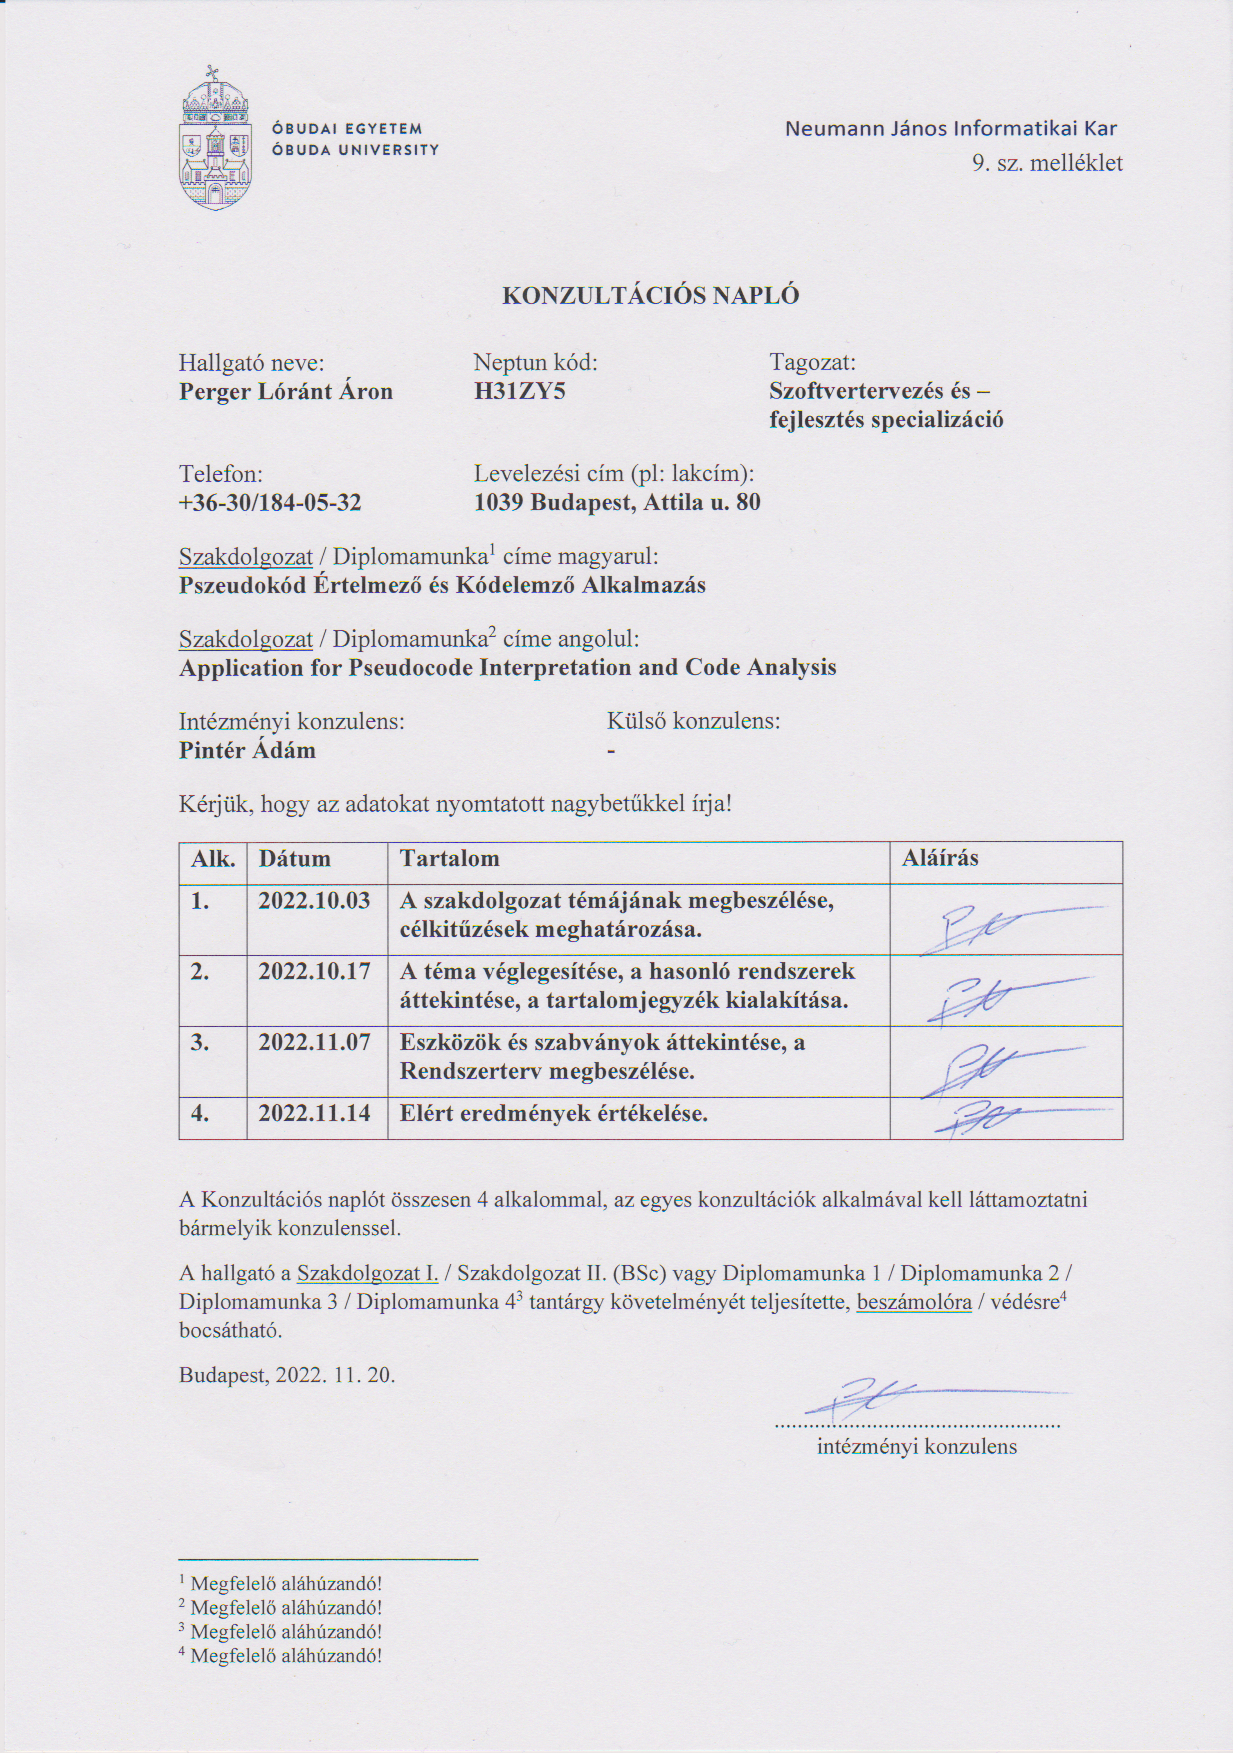
\includepdf[page=-]{img/elolapok/konzult1.png}
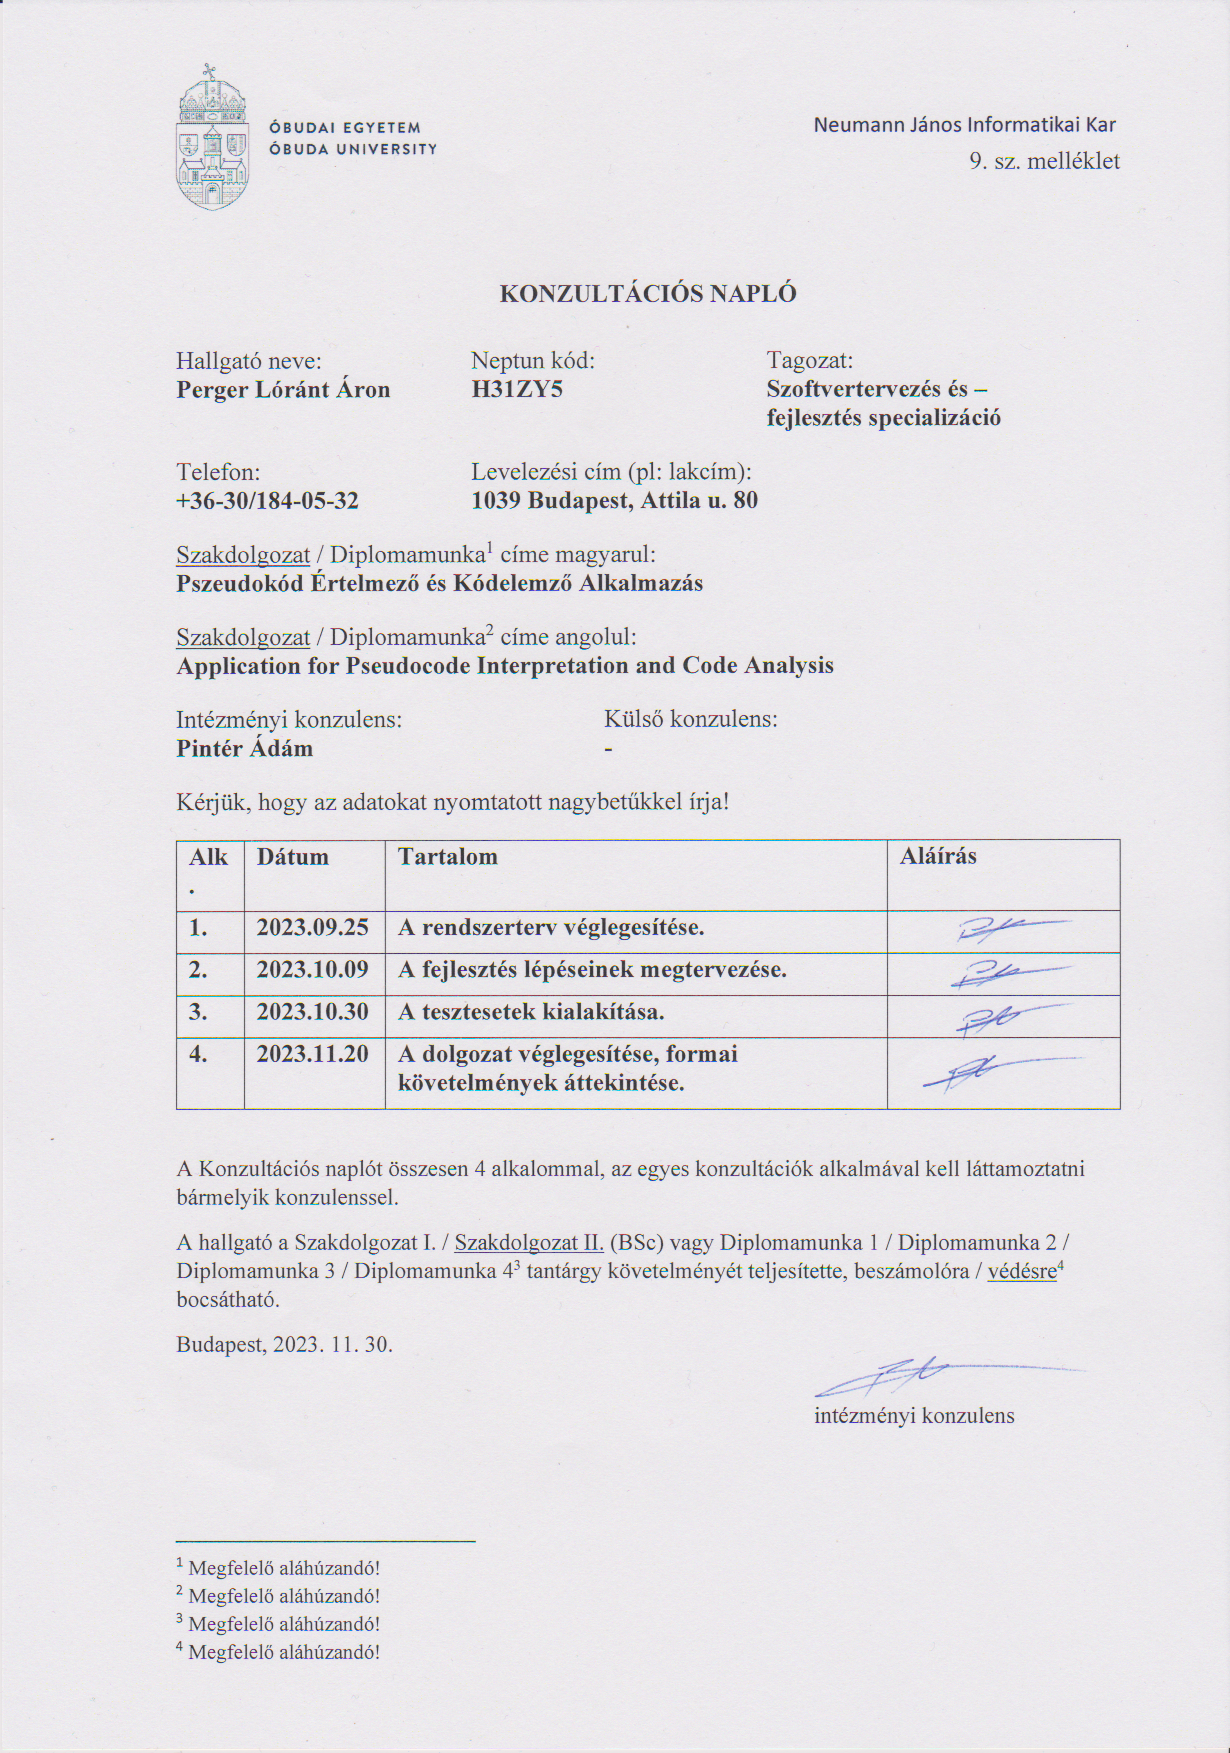
\includepdf[page=-]{img/elolapok/konzult2.png}

% -----------------------------------------------------

% ITT KELL HOZZÁADNI A FEJEZETEKET, CÍM NAGYBETŰVEL:

\clearpage
\section{ABSZTRAKT}

A következő szakdolgozat témája az Óbudai Egyetemen tanított, a programozás alapjainak demonstrálására használt Pszeudokód programozási nyelv és egy, a nyelvhez írt értelmezőprogram elkészítésének bemutatása. Célja, hogy dokumentálja és elmagyarázza egy programozási nyelv értelmezőjének megalkotását egy informális specifikációból kiindulva. Ehhez a nyelv szintaxisának és szemantikájának definiálása után sorra veszem a forráskód lefordításának lépéseit. Bevezetésre kerül a tokenizálás és az értelmezés fogalma, majd annak folyamata, hogy a fává alakított kódot hogyan tudjuk önálló lépésekre bontani. Ezután következik annak a virtuális gépnek definiálása, mely az előző fázisban kapott lépéseket végre is tudja hajtani és ezt oly módon a felhasználó elé tárni, hogy az belelásson a program belső működésébe és igény esetén a kódot megállítani és akár léptetni is tudja. A fogalmak és folyamatok leírása után bemutatok két egyéb fordítóprogramot és az elkészítésükhöz használt technológiákat, majd kiválasztom a saját projektemhez használt nyelvet. Végül a fordítás egyes lépéseit meg is valósítom, leírva azok gyakorlati működését a programomban. Az dolgozat végére egy olyan alkalmazás készül el, mely az egyetemen oktatott algoritmusokat képes végrehajtani és működésüket demonstrálni, ezáltal segítséget nyújtva az elsőéves hallgatók számára azok megértéséhez.

\clearpage
\section{ABSTRACT}

The following dissertation details the Pszeudokód ("Pseudocode") programming language taught at Óbuda University, along with the creation of a compiler capable of interpreting the language. The goal of the paper is to document and explain the process of creating a compiler when given an informal specification. I begin by describing the syntax and semantics of the language, followed by detailing the individual steps of transforming source code into a runnable state. I introduce the concepts of tokenizing and parsing, followed by the process during which the code's syntax-tree is unraveled into steps which can be individually executed. This is then followed by the introduction of a virtual machine, which is capable of running the instructions created during the last step in a way, that allows the user to monitor the algorithm's inner workings and, if need be, stop the program and execute instructions one by one. After describing these concepts and processes, I demonstrate two other compilers and their technologies, followed by choosing which language to use for my own project. Finally, I realize the steps described above, during which I explain their functionality and behavior specific to my program. By the end of this dissertation, the finished application is capable of interpreting and executing the algorithms taught at the university, and thus help first-year students understand them better.

\newpage
\tableofcontents
\newpage

% csak a tartalomjegyzék után kezdődik a számozás
\pagenumbering{arabic}

\clearpage
\section{BEVEZETÉS}
A szakdolgozatom témája egy az egyetemen tanított Pszeudokód értelmezésére és futtatására képes program, mely a beírt kód futtatására, léptetésére, az algoritmust futtató környezet belső információnak (változók, vermek és memória tartalma) kiíratására, és az algoritmusok végeredményének a kimenetre való kiírására.

A döntésem azért erre esett, mivel érdekelnek a programozási nyelvek és fordítóik működése és mivel az első félévben a programozás tárgy legnagyobb nehézségét a Pszeudokód megértése okozta.

Épp ezért döntöttem úgy, hogy olyasmit készítenék, ami kapcsolódik az érdeklődési körömhöz és reális haszonnal is rendelkezik, hisz egy ilyen program a későbbiekben segítséget nyújthatna a gólyáknak az algoritmusok megértésében.

A dolgozat először is specifikálja a Pszeudokód nyelv elemeit, szintaxisát, és működését. Ezután röviden bemutatom azokat az alapvető technikákat, amelyekből a programom felépül. Ezt követi pár hasonló program felületes összegzése, majd annak eldöntése, hogy melyik programozási nyelvet is fogom használni.

Ezt a program rendszerterve követi, mely nagy vonalakban specifikálja annak felépítését és a felhasználó által elérhető interfészét. Ezután következik a megvalósítás részletes leírása és annak tesztelése. Végül pedig a további esetleges fejlesztések felsorolása és a szakdolgozat összegzése.

\clearpage
\section{A PSZEUDOKÓD SPECIFIKÁCIÓJA}
\label{sec:specification}
Közel minden magyar, programozást tanító egyetemen, így az Óbudai Egyetemen is megtalálható egy Pszeudokódnak nevezett[17], legtöbbször C-re hasonlító képzeletbeli programozási nyelv. Ezek célja az algoritmusok egységesített alakba való átültetése és ezáltal a megtanulásuk megkönnyebbítése. Emellett pedig az olyan alapvető fogalmak megtanítása is, mint hogy mit jelent és miből áll a szintaxis, mik a típusok, mik a programok alkotóelemei és egyéb hasonlóképp kihagyhatatlan részei a programozó eszköztárának. Ebben a fejezetben specifikálni szeretném pontosan milyen elemekből is áll a Pszeudokód, milyen szintaxissal rendelkezik és milyen egyéb igényeket támaszt, melyet a dolgozatomnak el kell tudnia látni.

\subsection{Turing teljesség}
„A Turing-teljesség egy programozási- vagy lekérési nyelv vagy bármely más számítási modell erejéről szóló állítás, mely kijelenti, hogy bármit, amit egy Turing-géppel kiszámoltathatunk ezzel a nyelvvel vagy számítási modellel is ki lehet. Mivel a Turing-gépek a legerősebb eddig ismert számítási modell, így a Turing teljesség azt jelenti, hogy bármi ami egyáltalán kiszámítható, kiszámítható a nyelv használatával is. Ez a programozási nyelvek számára igencsak kívánatos tulajdonság, mivel ez azt jelenti, hogy a nyelv nem korlátozza a felhasználót abban, milyen problémát is oldhat meg vagy számítást fejezhet ki benne.”[6]

Ez a tulajdonság még azért is lényeges, mivel az ilyen nyelvekben leírt kód bizonyítottan bármely más Turing-teljes nyelvre átírható. Ahhoz, hogy a teljességet bizonyítsuk, meg kell mutatnunk, hogy a nyelv képes egy univerzális Turing-gépet szimulálni. Ez a képzeletbeli gép egy végtelen hosszú tekerccsel rendelkező olvasó/író fej, mely egy véges hosszúságú utasítási lista alapján képes a tekercsről adatokat beolvasni, majd ezeket értelmezve új adatokat írni arra (vagy a meglévőket felülírni.)

Mivel a Pszeudokód képes (elvben) tetszőleges hosszúságú tömbök létrehozására, ezekben a tömbökben véletlenszerű adatelérésre, módosításra és rendelkezik folyamatvezérlő szerkezetekkel, így kimondhatjuk, hogy a nyelv Turing-teljes és ezáltal bármely más tetszőleges ennek megfelelő nyelv kódját átfordíthatjuk rá vagy bármely Pszeudokódban írt program átfordítható egy másik ilyen nyelvre.

\subsection{Szintaktikai elemek és szemantikájuk}

A Pszeudokód sokat merít a C-szerű nyelvekből, így sok hasonlóság is felfedezhető benne. A következőkben a Pszeudokód szemantikai elemei és értelmezésük kerül bemutatásra.

\begin{code}{A Pszeudokód szintaktikai specifikációja}{code:syntax}
expression ::= arrayIndex | atom | binaryOperation | functionCall | not | reference | variable

statement ::= arrayComprehension | assignment | block | debug | for | functionCall | functionDeclaration | if | newArray | print | return | swap | while

block ::= statement+

newArray ::= variable " <- " (oneDimensionalArray | multiDimensionalArray)
multiDimensionalArray ::= "TáblaLétrehoz(" atomType ")[" expression ("," expression)+ "]"
oneDimensionalArray ::= "Létrehoz(" atomType ")[" expression "]"

swap ::= address " <- " address

if ::= ifHead (ifElseIf* ifElse)? " elágazás vége"

ifElseIf ::= ( " különben ha " expression " akkor " block)
ifElse ::= " különben " block
ifHead ::= "ha " expression " akkor " block 

for ::= "ciklus" variable "<-" expression ("-tól" | "-től") expression "-ig" block " ciklus vége"

while ::= normalWhile | doWhile
doWhile ::= "ciklus " block " amíg " expression
normalWhile ::= "ciklus amíg " expression block " ciklus vége"

return ::= "vissza " (expression | arrayComprehension) 

debug ::= "debug"

print ::= "kiír " expression

binaryOperation ::= logicOp

mulOp ::= primary | primary ("*" | "/" | "mod") primary
addOp ::= mulOp | mulOp ("+" | "-") mulOp
compOp ::= addOp | addOp ("<" | "<=" | ">" | ">=" | "=" | "=/=") addOp
logicOp ::= compOp | compOp ("és" | "vagy") compOp

primary ::= "(" expression ")" | not | reference | functionCall | arrayIndex | variable | atom

not ::= "~" expression
reference ::= "&" address

functionCall ::= functionName ("()" | "(" expression ("," expression)* ")")

functionDeclaration ::= "függvény " functionName ("()" | "(" parameter ("," parameter)* ")") statement+ " függvény vége"

functionName ::= [A-Z] ([a-z] | [A-Z])*

parameter ::= "címszerint "? (functionName | variable) " : " type

baseType ::= atomType | arrayType
arrayType ::= "rendezett "? atomType " tömb"
atomType ::= "egész" | "szöveg" | "logikai"


address ::= arrayIndex | variable

arrayIndex ::= variable "[" expression ("," expression)* "]"

variable ::= [a-z] ([a-z] | [A-Z])+

atom ::= string | number | boolean

string ::= '"' [a-z]* '"'
number ::= "0" | ( "-"? [1-9] [0-9]* )
boolean ::= "Igaz" | "igaz" | "Hamis" | "hamis"

nl ::= " "* "\n"+ " "*

\end{code}

\subsection{Függvények és eljárások}

A Pszeudokód különbséget tesz a függvények és eljárások között. Az előbbi visszatér értékkel, az utóbbi nem. Mindkettő a 1. kódnál szereplő szignatúrát követi:

Az Óbudai Egyetemen használt Pszeudokódok része, hogy a sorok elején az olvasás és idézés egyszerűbbé tételének kedvéért számokat helyezett el az író.

Ezt pusztán az olvasó számára szolgál valós információval, a nyelv önmaga nem rendelkezik se GOTO utasítással, se más egyéb szerkezettel mellyel sorszámalapú ugrást tudnánk végrehajtani, így az én megvalósításomban is ezek figyelmen kívül lesznek hagyva.

\subsection{Kimenet/Bemenet sorok}

Minden Pszeudokód algoritmus első két sora arra való, hogy definiálja a be- és kimeneti változókat, mellyel az algoritmus dolgozik. Ez a 2.2-es forráskódban látható.

Mivel mind a bemeneti, mind a kimeneti változók kiderülnek a függvény szignatúrájából és visszatérési értékéből, így az én megvalósításomban ezek figyelmen kívül lesznek hagyva.

\subsection{Visszatérési értékek}

A Pszeudokód a C-szerű nyelvekkel ellentétben támogatja a több értékkel való visszatérést. Tehát egy érték helyett, akár kettővel, hárommal vagy elméletileg többel is visszatérhetünk a függvényekből.

A helyzetet még az komplikálja, hogy bizonyos esetekben más számú visszatérési értékekkel kell számolnunk. Ez legtöbbször például a kereső függvényeknél van használva, ahol az első érték azt jelzi, hogy egyáltalán megtaláltuk-e a keresett értéket, míg a második ennek indexével tér vissza, ha igen. Ilyen esetekben, ha nem találtunk megfelelő értéket egy darab visszatérési értékkel rendelkezünk, ha igen, akkor pedig kettővel.

Mivel a Pszeudokód támogatja a tömböket, így több értékkel való visszatérés esetén egyszerűen egy tömböt adunk vissza.

\clearpage
\section{FELHASZNÁLT TECHNIKÁK, MÓDSZEREK}
\label{sec:techniques}
A program egy egyszerű interpreter, így az ilyen alkalmazásoknál megszokott összetevők itt is megjelennek.

\subsection{"Lexer"—Lexikai analízis}

„Az első lépés bármely értelmező vagy fordító létrehozásában a szkennelés1. A szkenner a nyers bemeneti forráskódot karakterek sorozataként fogadja, majd ezeket tokeneknek nevezett csoportokba gyűjti. Ezek a nyelv értelmes »szavai« és »írásjelei« melyek kialakítják annak nyelvtanát.”[2]

A tokenek közé tartoznak például az operátorok, a változónevek, a különböző utasítások és kifejezések nevei, és az úgynevezett „atomok,” melyek olyan értékek, amik például számokat vagy szövegeket tartalmaznak.

A Lexer feladata ezen kívül még az úgynevezett „triviák”, avagy jelentéssel nem bíró elemek megszüntetése is. Ezek közé tartoznak a kommentek (hisz ezeket az értelmező figyelmen kívül hagyja) és az jelentést nem módosító üres helyek (mivel a program szempontjából nem jelent semmiféle különbséget, hogy valaki „5 + 3”-t ír vagy „5          +3”-t vagy mindhárom karaktert különböző sorba írja).

Mivel a lexikai analízis egy elég szimpla és túl sok változatosságot nem mutató folyamat, így kevés hozzá kapcsolódó, néven nevezett algoritmus létezik. A fő befolyásoló elem az a nyelv maga, amelyben az interpreter van írva. Ha rendelkezünk reguláris kifejezésekkel2, az nagyban megkönnyítheti a munkát, hisz a legtöbb lexikai szabály egy-az-egyben kifejezhető ilyenek segítségével.

Az egyetlen hibakezelés, melyet ebben a szekcióban végzünk az értelmetlen tokenek szűrésére vonatkozik. Mivel a lexernek nincs tudása arról, hogy ezeknek milyen sorrendben is kell követniük egymást, ezért például hiba nélkül el fog fogadni egy olyan kódot, mely a következőképp szól „ha amíg x+5” annak ellenére, hogy ez nyilvánvalóan hibás kód. Viszont, ha olyasmit írunk, hogy „ha --” azt már ebben a lépésben is ki tudjuk szűrni, hisz a nyelv nem támogatja a csökkentő operátort.

Feltéve, hogy a bemenetünk nem hibás a lexer a következő lépéseket hajtja végre:

\begin{enumerate}

    \item Ellenőrzi, hogy a bemenet végére értünk-e. Ha igen, visszatér a tokenek listájával.

    \item Ha nem, akkor átugorja az úgynevezett triviákat, ezek a fentebb tárgyalt jelentéssel nem rendelkező elemek (kommentek, többszöri üres helyek, többszöri új sor nyitása.)

    \item Izolálja a következő tokent, a következő módon:

    \begin{enumerate}

        \item Operátorok („+”, „-”, „/” „x”, „←”, „<=”, „>=”, „=”, „=/=”) esetén ez egy, kettő vagy három karaktert jelent. Ez nem okoz problémát, hisz az operátor első (vagy az utolsó operátor esetén az első és a második) karaktere egyértelművé teszi, milyen fajta is.

A lexernek nem feladata, hogy az operátorok precedeniáját (tehát a számítások matematikai szabályok szerinti sorrendben történő kiszámítását) figyelembe vegye. Erről a parser felel.

        \item Kulcsszavak esetén csak egyszerűen végigiterálunk egy listán, mely az összes kulcsszót tartalmazza és visszatérünk, ha bármikor egyezést találunk.

        \item Egyébként a token egy atom, mely szám esetén nem igényel egyéb módosítást, szöveg esetén viszont szükséges az idézőjelek levágása a végeiről.
    \end{enumerate}

    \item A lexer létrehoz egy új tokent, beállítja a fajtáját és ha rendelkezik egyéb adattal (például atomok esetén), akkor azt is beállítja az erre a célra kijelölt mezőben.

    \item A lexer hozzáadja a listához a tokent, majd a visszalép az első lépésre.

\end{enumerate}

Az így kapott lista ezután továbbításra kerül a következő egységhez, az értelmezőhöz.

\subsection{"Parser"—Értelmezés}

A „parser” vagyis értelmező feladata az előző lépésben készített tokenekből a gép számára is értelmezhető formátumot alkotni. Ezt egy úgynevezett „absztrakt szintaxisfával” reprezentáljuk, mely egy tokenekből alkotott fa, melynek levelein csak atomok találhatóak, ágain pedig egy vagy több értéket fogadó operátorok és kulcsszavak állnak.

A parser felelős azért is, hogy a statikus szintaktikai hibákat kiszűrjük. Ide tartoznak az egymást nem követhető kulcsszavak, a kulcsszavakhoz való értékadás, hiányzó lezáró tokenek („elágazás vége” hiánya), két egymás utáni atom és bármely egyéb olyan kódszerkezet, amelynek nincs értelme a nyelv specifikációja szerint.

A lexerekkel ellentétben számos parser létezik, alább szeretnék kettőt jellemezni, amelyek a leginkább hasznosnak tűnnek számomra.

\subsubsection{Rekurzív alászálló parser}

A rekurzív alászálló parserek[19] egy felülről-lefelé haladó parser, mely rekurzív procedúrákkal dolgozza fel a tokeneket.

Két fő fajtáját különböztetjük meg az ilyen parsereknek. Az első egy bizonyos véges számú token alapján képes eldönteni pontosan milyen szerkezetnek kell a szintaxisfába kerülnie.

A másik egymás után próbálgatja a szabályokat, amíg vagy a lista végére nem érünk (mely esetben hibát dobunk) vagy találunk egy olyan szabályt, mely illeszkedik a tokenekre.

\subsubsection{PEG parser}

A PEG parser[3] nagyban hasonlít a sima alászálló parserekhez, viszont azokkal ellentétben minden egyes illeszkedő szabály minden esetben garantáltan megadja pontosan milyen értéket is talált a parser. Emiatt nagyon hasznos programozási nyelvekhez és így ezt szeretném használni a projektemben.

\subsection{Virtuális Gép—Végrehajtás}

A „virtuális gép” egy olyan program, melynek feladata, hogy a parser által generált szintaxisfát lefuttassa, úgy mintha az egy képzeletbeli, egyszerűsített számítógépen futna. A felhasználó számára talán ez a „legizgalmasabb” része a programnak, hisz amint ez a része véget ér jelenik meg a képernyőn a kód végeredménye.

A virtuális gép lényegében egy minden érvényes utasítást értelmezni képes switch elágazásból; egy változókat és a nyelven belül definiált függvényeket számon tartó adatszerkezetből (melyet környezetnek nevezünk) és valamilyen futási hibakezelésből áll.

A virtuális gép működésének egyik megközelítése a rekurzió, hisz a szintaxisfánk egy fa, melynek minden ága is egy értelmes szintaxisfának felel meg. Így alkalmas stratégia, hogy egészen addig osztogatjuk fel részproblémákra a futtatást, míg a levelekig nem érünk, melyek nem igényelnek semmiféle feldolgozást. Innentől pedig a rekurzió elkezd visszafejleni és a levelek fölötti ágak eredményei válnak az új levelekké.

Az \ref{fig:aritmast} ábra bemutatja a 10 / 2 * 15 + 5 egyenlet kiszámolását egy egyszerű szintaxisfa segítségével.

\addimage{ast.png}{Példa egy absztrakt szintaxisfára.}{aritmast}

A futtatás akkor ér véget, ha vagy a szintaxisfa legvégére értünk vagy hibába ütköztünk. 

Másik megközelítés, hogy ezt a fát először egy tömbbé változtatjuk, melynek utasításai nem függenek egymástól. Ennek előnye, hogy a futtatás bármikor megállítható, a rekurzív megközelítéssel szemben, melynél muszáj egy végeredményt kiértékelnünk mielőtt az algoritmus megállna. 

A saját megvalósításomban ezt az utóbbi megközelítést választottam, mivel így csupán még egy rétegnyi feldolgozás bevezetésével a kód léptethetővé és futás közben változtathatóvá válik. Ennek részleteiről a megvalósításról szóló fejezetben írok.

Mivel a projektspecifikáció része, hogy léptetni is lehessen a kódot előre- és visszafelé is, emiatt a gép állapotát és az egyes környezeteket érdemes úgynevezett megváltoztathatatlan („immutable”) adatszerkezetekben eltárolni, így léptetés esetén csak a jelenleg aktív szerkezetet cseréljük ki egy korábbi vagy újabb verzióra.

\clearpage
\section{HASONLÓ TECHNOLÓGIÁK BEMUTATÁSA}
\label{sec:similar}
Az alábbi fejezetben szeretném bemutatni azokat a nyelveket és implementációjukat, melyek segítettek a téma megértésében.

\subsection{Brainf**k}

\subsubsection{A nyelvről röviden}

A Brainf**ck (BF) egy úgynevezett „ezoterikus programozási nyelv,” mely annyit jelent, hogy nem valós használatra szánták, hanem szimplán viccből vagy valami érdekes megkötés vállalásával alkották. A nyelv érdekessége, hogy összesen nyolc utasítást tartalmaz, melyek mind egy-egy karakterből állnak, ennek ellenére a nyelv Turing-teljes és elméletileg bármely más Turing-teljes nyelven megoldott probléma átültethető bele, bár ez a nyelv különleges szintaxisa miatt felettébb nehéz.

Azért választottam ennek a nyelvnek a bemutatását, mivel ez az egyik legkisebb olyan nyelv, amit nagyon egyszerűen megvalósíthatunk, de mellé megtanítja a nyelvkészítés alapjait.

A BF működési elve egy, a Turing-géphez hasonló, cellákra felosztott szalag, mely egyszerre a program által felhasznált adatokat tartalmazza és egy külön lista, mely a program által végrehajtott utasításokból áll. Ezen kívül rendelkezik egy képzeletbeli „fejjel,” mely mindig az adatokat tároló szalag egyik cellájára mutat. Ez a fej felelős az adatok írásáért és olvasásáért, programozási analógiával élve a szalag egy hosszú, számokat tartalmazó tömb, a fej pedig a tömb egyik elemére mutató pointer.

A nyelv a következő utasításokat érti:

\begin{itemize}
    \item \textbf{<} - Egyel balra lépteti a fejet a szalagon.
    \item \textbf{>} - Egyel jobbra lépteti a fejet a szalagon.
    \item \textbf{+} - Egyel megnöveli a jelenlegi cella értékét.
    \item \textbf{-} - Egyel csökkenti a jelenlegi cella értékét.
    \item \textbf{[} - Ha a fej alatti érték nulla előreugrik a következő ] karakterhez az utasításokban. Ellenkező esetben szimplán tovább lép a következő utasításra. 
    \item \textbf{]} - Ha a fej alatti érték nem nulla, visszaugrik az előző [ karakterhez az utasításokban, különben tovább lép a következőre.
    \item \textbf{,} - Beolvas egy bájtot a bemenetről és eltárolja a szalag jelenlegi cellájában.
    \item \textbf{.} - Kiírja a fej alatti cella értékét a standard kimenetre karakterként értelmezve.
\end{itemize}

Egy egyszerű BF program, mely összead két számot: \verb|[->+<]|

Tehát addig hajtjuk végre ezeket az utasításokat, míg az első cellában lévő szám nullává nem válik úgy, hogy egyel csökkentjük az első cella értékét, majd jobbra lépünk, a jobboldalit egyel növeljük, majd visszalépünk az eredetire.

\subsubsection{Projekt bemutatása}

A nyelvre írt interpreter bemutatásához egy C nyelvben írt egyszerű interpretert[9] szeretnék felhasználni, mely emellett egy API-t is elérhetővé tesz a felhasználó számára, mellyel más projektekbe is beépíthetővé válik az értelmező.

A program belépés után ellenőrzi milyen közegben is lett meghívva és ennek alapján tölti be a kódot vagy egy fájlból vagy a standard bemenetről (vagy dob hibát hibás meghívás esetén.) Az egyszerűség kedvéért én a standard bemenetről történő beolvasást fogom végigvezetni, hisz a program többi funkcionalitása (fájlkezelés, szövegbeolvasás közben történő hibakezelés) számunkra nem releváns. A bemutatott kód egésze a 4.1-es forráskódban látható.

Az első sor inicializál egy üres láncolt listát, mely az utasításokat fogja tartalmazni. A második pedig egy üres 30.000 hosszúságú tömböt inicializál, ez lesz az szalagunk. 

Ezután belépünk a brainfuck\_parse\_string függvénybe, mely egyszerre végzi a Lexer és a Parser feladatát. A függvény átlépked az utasításokon és úgy csoportosítja a jobbra -balra lépéseket, a beolvasást és kiírást és a növelést-csökkenést, hogy az ugyanolyan fajtájúak egy-egy instrukcióvá változnak. Például, ha egymás után három pluszjelet lát a program, akkor ahelyett, hogy a szalag értékét háromszor egyel növelné, helyette egy olyan instrukciót helyez el, mely hárommal növeli az értéket egyszer. Ezen kívül, ami érdekes még, az az, hogy a szögletes zárójelek által definiált ciklusok külön beágyazott fákként jelennek meg a végső szintaxisfában.

Ezután az így kapott fát behelyezzük az utasításokat tartalmazó listába és lefuttatjuk. Mivel a BF utasításai remekül illeszkednek az egyszerű tömb/pointer műveletekre így a legtöbb elem szimplán egy sorrá átalakítható.

Végül pedig felszabadítjuk mind az utasítás, mind az adatok listájának memóriáját és sikerrel visszatérünk.

\subsection{Rockstar}

\subsubsection{A nyelvről röviden}

A Rockstar\cite{rockstar} egy paródia programozási nyelv, mely különlegessége, hogy a nyelven írt kód az elmúlt évtizedek Rock és Metál szövegeire emlékeztet. A nyelv a BF-hez hasonlóan szintén Turing-teljes, bár annak ellenére, hogy nem általános programozásra alkották sokkal inkább használható. A nyelvet Dylan Beattie alkotta, akit egy Twitteren olvasott üzenet ihletett meg.

A nyelv specifikációja megtalálható a Github tárolóján1, így én nem szeretnék erre külön kitérni, kivéve, ahol ez szükséges. Én a nyelv referencia implementációjára szeretnék most fókuszálni, mely egy JavaScriptben írt értelmező, mely a böngészőn belül és azon kívül is működik.

\subsubsection{Projekt bemutatása}

A referencia implementáció, mely a Satriani névre hallgat egy PEG.js nevű könyvtárat használ a Parser legenerálására.

„A PEG.js egy egyszerű JavaScript parser generátor, mely gyors parsereket generál remek hibaüzenetekkel. Bonyolult adatok feldolgozására, programozási nyelvekhez, fordítói rendszerekhez, értelmezőkhöz, fordítókhoz és egyéb eszközökhöz is egyszerűen használható.”[8]

Az ebből kapott szintaxisfát egy aránylag szimpla virtuális gép futtatja, mely két fő részből áll: Egy Environment-nek nevezett adatstruktúrából, mely a változókat és az egyéb, futtatáshoz szükséges, információkat tartalmazza és egy hosszú switch-elágazásból, mely végrehajtja a szintaxisfa utasításait.

\clearpage
\section{A MEGVALÓSÍTÁSHOZ HASZNÁLT NYELV}
\label{sec:language}
Bár az interpreterek nem triviális programok, mégis szinte bármely programnyelv felhasználható az implementálásukra. Mivel szeretném, hogy a projektmunkám webes felületen is elérhető legyen, így ezt a funkcionalitást mindenképp figyelembe kell vennem, amikor a nyelveket értékelem.

Ideális esetben a nyelv rögtön weben is futtatható állománnyá fordul, ám mivel a legtöbb programozási nyelv nem képes ilyesmire, ezért jó lehetőségnek kínálkozik az úgy nevezett WebAssembly-re való fordítás.

„A WebAssembly (rövidítve Wasm) egy biztonságos, hordozható, és alacsony-szintű kódformátum, melyet gyors futtatásra és kompakt méretű ábrázolásra terveztek. A fő célja, hogy lehetővé tegyen gyorsan futtatható programokat a Weben, anélkül hogy bármilyen Web-irányú feltételezést tenne vagy Web-specifikus funkciókat tenne lehetővé, ezáltal más közegekben is használhatóvá váljon.”[20]

Alább szeretném kifejteni melyik nyelveket vettem fontolóra:

\newpage

\subsection{C}

Természetesen nem hagyhatjuk ki az egyik legöregebb és mégis széles körűen használatos nyelvet.

A C pozitívumai közé sorolandó, hogy nagyon könnyen lehet más platformokra fordítani. Az Emscripten nevű fordítói csomag segítségével a C Wasm formátumba is fordítható, ezáltal böngészőben is futni képes.

„Az Emscripten egy nyílt-forráskódú fordító WebAssembly-re. A segítségével C és C++ kódot vagy bármely más LLVM-et használó nyelvet WebAssembly-re fordíthatunk és az Web-en, Node.js-en, vagy más wasm futtatási környezetben futtathatjuk.”[4]

A nyelv pozitívumai közé sorolandó még, hogy nem túl „meglepő” (kevés szintaxissal és aránylag átlátható szabályokkal rendelkezik), kifejezetten gyors és kis állományokká fordul, és szinte páratlan szabadságot ad a fejlesztőnek a rendszer erőforrásainak felhasználásához.

Cserébe  viszont a több évtizedes standard könyvtár és a nyelv pár furcsasága miatt könnyen futhat a programozó furcsa hibákba, mint például a szövegeknél esetlegesen hiányzó null byteok esetén történő túlcsordulások, vagy a hibásan lefoglalt / korábban felszabadított memóriaterületekre való írás/olvasás esetén előforduló végzetes hibák.

Ezen kívül a teljesen manuális memóriakezelés bár nagyon hasznos tud lenni, de jelen problémához fölösleges plusz terhet jelent csak. Ezen kívül a nyelv nem támogatja az osztályokat, helyette struct-ok átadogatásával oldjuk meg az egybefüggő objektumok megváltoztatását. Ez sajnos nagyon könnyen tud átláthatatlansághoz vezetni, mely egy ilyen nem-triviális projektnél elfogadhatatlan.

Bár a nyelv az egyik személyes kedvencem, számomra nem megfelelő a feladathoz. A nyelv értékelésének összefoglalója az \ref{cnyelv} táblázatban látható.

\begin{center}
  \captionof{table}{A C nyelv értékelése.\label{cnyelv}}
  \begin{tabularx}{\textwidth}{X X}
    \hline
    \multicolumn{1}{c}{\bfseries{Pozitívumok}} & \multicolumn{1}{c}{\bfseries{Negatívumok}}                                  \\
    \hline
    Könnyen fordítható Wasm-be                 & Manuális memóriakezelés                                                     \\
    Jól felszerelt eszköztár                   & Nincs OOP                                                                   \\
    Személyes ismeretség                       & Kényelmi funkciók hiánya (pl.: regex, for-each, map, adatszerkezetek, stb.) \\
    Más nyelveket is ebben írtak (pl.: Python) & Nincs könnyű mód a hibakezelésre (segfault)                                 \\
    \hline
  \end{tabularx}
\end{center}

\newpage

\subsection{C++}

A C++ kijavítja a C főbb hibáit a RAII-vel (Resource Aquisition Is Initialization[18], „az erőforrás lefoglalása egyben inicializáció is,” magyarul a különböző adattagok létrehozásakor a memória automatikusan lefoglalódik, megszűnésükkor pedig felszabadul) és egy sokkal kevésbé meglepő standard könyvtárral, viszont cserébe új negatívumokat ad az egyenlethez.

Bár az Emscripten képes Wasm formátumba fordítani a nyelvet, a hibakezelése problematikus. Alapesetben a generált kód végzetes hibával lép ki bármilyen hiba esetén, beleértve az amúgy elkapható exception-öket. Ugyan egy kapcsoló segítségével engedélyezhetjük, hogy az utóbbi hibák újra elkaphatóak legyenek, ez súlyos lelassuláshoz vezet a programban.[5]

Ezen kívül a szövegkezelése a lentebb tárgyalt nyelvekhez képest igen nehézkes. Bár vannak regex könyvtárak, de ezekkel kapcsolatban semmi ismeretségem nincs. A C++ rendelkezik hibakezeléssel, viszont ennek ellenére dobhat segfaultot1. A nyelv nem rendelkezik hivatalos csomagkezelővel sem, így a könyvtárak beimportálása nem feltétlen egyszerű és nem garantált, hogy ezek valóban át is fordulnának Wasm-ra.

Mivel a nyelv használhatósága ennyire kétséges, így nem felel meg számomra a feladathoz. A nyelv értékelésének összefoglalója az \ref{cppnyelv}-es táblázatban látható.

\begin{center}
  \captionof{table}{A C++ nyelv értékelése.\label{cppnyelv}}
  \begin{tabularx}{\textwidth}{X X}
    \hline
    \multicolumn{1}{c}{\bfseries{Pozitívumok}}         & \multicolumn{1}{c}{\bfseries{Negatívumok}}                                             \\
    \hline
    Van OOP                                            & Bár van hibakezelés, de segfaultok itt is történhetnek                                 \\
    RAII (memóriakezelést leegyszerűsíti)              & A szövegkezelés nehézkes (stream-ek, atoi és hasonló átalakító függvények furcsaságai) \\
    Ésszerű, kiforrott standard könyvtár               & A WebAssemblybe való fordítás lassú és több előkészületet igényel                      \\
    Személyes tapasztalat (bár nem annyi mint a C-vel) & Nem minden külső könyvtár alkalmas a Wasm-ba való fordításra                           \\
    \hline
  \end{tabularx}
\end{center}

\newpage

\subsection{C\#}

„A Blazor a Microsoft új kísérletbeli framework-je, mely pluginok használata nélkül hozza el a C\#-ot bármely böngészőbe.”[11] Az előző két nyelvvel ellentétben a C\# teljesen automatikus memóriakezeléssel rendelkezik, ezen kívül a C++-hoz hasonlóan ugyanúgy lehet benne osztályokat és interfészeket használni, mely által a kód sokkal átláthatóbb.

Viszont míg a többi nyelvnél a kliens maga képes a kód teljes feldolgozására és lefuttatására, a Blazor használatánál szükséges egy szervergép is, melyet fel kell szerelnünk a szerver futtatásának minden szükséges elemével (megfelelő hardver, .NET Core telepítése.)

Bár az egyetemi tanulmányaim miatt sok tapasztalattal rendelkezem már a nyelvvel kapcsolatban, nem szívesen kötném magam egy webes frameworkhöz, így a C\# sem megfelelő számomra a feladathoz. A nyelv értékelésének összefoglalója az \ref{csnyelv}-as táblázatban látható.

\begin{center}
  \captionof{table}{A C\# nyelv értékelése.\label{csnyelv}}
  \begin{tabularx}{\textwidth}{X X}
    \hline
    \multicolumn{1}{c}{\bfseries{Pozitívumok}}                              & \multicolumn{1}{c}{\bfseries{Negatívumok}}                      \\
    \hline
    Sok személyes tapasztalat                                               & Terjengősebb mint a többi nyelv                                 \\
    A memóriakezelést a rendszer intézi, nekünk nem kell foglalkoznunk vele & Semennyi tapasztalatom nincs a webes frameworkökkel             \\
    Blazor framework kifejezetten webes alkalmazások fejlesztésére          & Futtatási környezetet igényel, nagyobb mint a fentebbi nyelvek. \\
    Kiváló standard könyvtár                                                                                                                  \\
    Erős OOP                                                                                                                                  \\
    Jó szövegkezelés                                                                                                                          \\
    \hline
  \end{tabularx}
\end{center}

\newpage

\subsection{LiSP}

A LiSP[16] egy C-hez hasonló korú nyelv, mely lényege, hogy a kód és az adat ugyanolyan adatszerkezetben vannak tárolva. Ez nem más, mint a láncolt lista, mely lehetővé teszi, hogy bármilyen hosszúságú és bonyolultságú adatot el tudjunk tárolni aránylag egyszerű módon.

Bár egyáltalán nem tartom megfelelő nyelvnek a projektemhez, nem hagyhattam ki a megemlítését, hisz a láncolt lista futtatása nagyon hasonlít a virtuális gépről szóló fejezetben tárgyalt működéséről.

A Structure and Interpretation of Computer Programs\cite{sicp} című könyv sokat segített a folyamat megértésében, mely a LiSP egyik átalakított változatát, a Scheme-t használja és egy fejezetében egy interpreter majd később egy fordító megírását mutatja be. A nyelv értékelésének összefoglalója az \ref{lispnyelv}-ös táblázatban látható.

\begin{center}
  \captionof{table}{A LiSP nyelv értékelése.\label{lispnyelv}}
  \begin{tabularx}{\textwidth}{X X}
    \hline
    \multicolumn{1}{c}{\bfseries{Pozitívumok}}               & \multicolumn{1}{c}{\bfseries{Negatívumok}}              \\
    \hline
    A kód maga egyben adat is                                & Semmi reális tapasztalatom nincs a nyelvvel             \\
    Nem igényel fordítást, gyorsan lehet prototípizálni vele & Idegen, nehezen átlátható szintaxissal rendelkezik      \\
    Páratlan listafeldolgozási képességekkel rendelkezik     & Nem igazán interneten át való futtatásra kitalált nyelv \\
    Kiforrott standard könyvtárral rendelkezik               & Nem szeretném használni                                 \\
    \hline
  \end{tabularx}
\end{center}

\newpage

\subsection{Rust}

„A Rust programozási nyelv segít, hogy gyorsabb és megbízhatóbb szoftvert írjunk. A magas-szintű ergonómia és az alacsony-szintű irányítás gyakran összeegyeztethetetlen a programozási nyelvek dizájnjában; a Rust ezt az állítást kérdőjelezi meg.”[7]

A Rust egy relatíve új programozási nyelv, mely céljának a teljes memória-biztonságot és a gyakori hibák elkerülését tűzte ki, emellett natív fordításra is képes. A statikus analízise erősebb az összes fentebb felsorolt nyelvnél, a sebessége pedig a C/C++-hoz hasonlatos. Ezen kívül remek könyvtárakkal rendelkezik, melyek például a regexelést nagyon egyszerűvé teszik. A nyelv natívan fordul WebAssembly-re így ez se okoz problémát.

Cserébe a nyelv írása nagyon nehézkes, a fordító ott ahol tud felhívja a figyelmét a programozónak az esetleges hibákra vagy kifelejtett ellenőrzésekre. Ez természetesen a program minőségére nézve abszolút pozitív, ám cserébe nagyon nehézkessé teszi a prototípusok létrehozását.

Mivel a nyelv használata ilyen nehézkes és a prototípizálás lassú, így nem szeretném ezt a nyelvet választani. A nyelv értékelésének összefoglalója az \ref{rustnyelv}-os táblázatban látható.

\begin{center}
  \captionof{table}{A Rust nyelv értékelése.\label{rustnyelv}}
  \begin{tabularx}{\textwidth}{X X}
    \hline
    \multicolumn{1}{c}{\bfseries{Pozitívumok}}         & \multicolumn{1}{c}{\bfseries{Negatívumok}} \\
    \hline
    Gazdag standard könyvtár                           & Nehézkes szintaxissal rendelkezik          \\
    Jó hibakezelés, segfault átlagos kódban lehetetlen & Nincs vele elég tapasztalatom              \\
    Remek könyvtárak, csomagkezelővel                  & Fordítás kicsit lassú                      \\
    Natív fordulás böngésző által is érthető formátumba                                             \\
    \hline
  \end{tabularx}
\end{center}

\newpage

\subsection{JavaScript}

Mivel a program követelményei közé tartozik, hogy internetről elérhető felületen lehessen használni, így a böngészőkben natívan futó JavaScript kifejezetten alkalmas jelölt a szakdolgozat elkészítésére.

Ám, mivel nagyon kevés garanciát biztosít a rosszul használt típusok és egyéb programozói óvatlanságból eredő hibák elkerülésére, így mégse erre esett a választásom, hanem az egyel lentebbi szekcióban taglalt TypeScript-re. A nyelv értékelésének összefoglalója az \ref{jsnyelv}-es táblázatban látható.

\begin{center}
  \captionof{table}{A JavaScript nyelv értékelése.\label{jsnyelv}}
  \begin{tabularx}{\textwidth}{X X}
    \hline
    \multicolumn{1}{c}{\bfseries{Pozitívumok}}             & \multicolumn{1}{c}{\bfseries{Negatívumok}}                    \\
    \hline
    A legegyszerűbb szerverről felszolgálható              & Lassabb mint egy fordított nyelv                              \\
    A végfelhasználónak csak böngészővel kell rendelkeznie & A legtöbb rossz típusból eredő hiba csak futás során derül ki \\
    Dinamikus tömbökkel és automatikus memóriakezeléssel rendelkezik                                                       \\
    Kiforrott eszközökkel rendelkezik, melyek segítségével a hibák száma és a kód mérete minimalizálható                   \\
    \hline
  \end{tabularx}
\end{center}

\newpage

\subsection{TypeScript}

„A TypeScript egy erősen típusos programozási nyelv, mely a JavaScriptre épül és bármely kódméret esetén jobb eszközkészletet nyújt.”[10] Mivel nem igényel valódi fordítást, ezért nagyon gyorsan lehet vele prototípusokat gyártani és a program futtatása szinte semmi előfeltételt nem igényel egy böngészőn túl.

Viszont mivel a TypeScript alatt futó JavaScript dinamikus típusokkal rendelkezik és az általa futtatott analízis csak a deklarált típusok pontosságát ellenőrzi, így nem képes a futási hibák kiszűrésére. Ennek ellenére a vizsgált nyelvek közül ez bizonyult annak, amely egyrészt kevés eszközt igényel, másrészt pedig rögtön böngészőben is futtatható formátumot produkál, így a választásom erre a nyelvre esett.

A nyelv értékelésének összefoglalója az \ref{tsnyelv}-es táblázatban látható.

\begin{center}
  \captionof{table}{A TypeScript nyelv értékelése.\label{tsnyelv}}
  \begin{tabularx}{\textwidth}{X X}
    \hline
    \multicolumn{1}{c}{\bfseries{Pozitívumok}} & \multicolumn{1}{c}{\bfseries{Negatívumok}}                                               \\
    \hline
    Natívan az interneten futó kód             & Gyengébb típusellenőrzés mint egy normálisan fordított nyelvben                          \\
    Sok személyes tapasztalat                  & Lassabb lehet mint a fentebbi nyelvek                                                    \\
    Nagyon gyorsan prototípizálható nyelv      & Mivel a TS alatt futó JS dinamikusan típusos emiatt könnyen lehet váratlan hibákba futni \\
    Jó szövegkezelés (beépített regex)         & A nyelv OOP-je nem kifejezetten kiforrott                                                \\
    Automatikus memóriakezelés, extra védelmek a böngészőben való futás miatt                                                             \\
    \hline
  \end{tabularx}
\end{center}

\clearpage
\section{RENDSZERTERV}
\label{sec:plan}
\subsection{Összeállítás}

A diplomamunka egyes elemei külön egységekként lesznek lekódolva, melyek interfészekkel lesznek képesek egymással kommunikálni. Ez azért ideális, mert a végeredmény egy nagyon kevés fájlból álló, egyszerűen mozgatható és felállítható csomag, viszont az eredeti forrásállományok egymással való nem függése miatt könnyű bármelyik részt lecserélni, ha ez esetleg szükségessé válna.

Mivel a fent felsorolt nyelvek majdnem mind képesek natív formátumba is fordulni, ezért amíg el nem érünk a felhasználó interfész kialakításához, a kód helyileg is tesztelhető, akár egy nyelvre specifikus unit teszt frameworkkel, akár valamely automatizált módszer segítségével.

A külső könyvtár által generált szintaxisfát egy általam írt átalakító osztályban használom fel, mely képes rekurzív adatstruktúrából tömbszerűt alkotni. Ez utána egy futtató osztályba kerül, mely a felhasználói felülettel kapcsolatban áll oly módon, hogy annak információkat küld és attól parancsokat fogad. Ennek folyamatát a 6.1-es ábra mutatja be.

Mivel a program egyszerű JavaScriptből és HTML+CSS fájlokból áll és letöltés után a végfelhasználó számítógépén fut, így szinte bármilyen interneteléréssel és statikus fájlokat elérhetővé tenni képes szerverrel felszerelt gépről felszolgálható.

\subsection{Felhasználói interfész}

Mivel a projekt célja, hogy a Pszeudokód megértéséhez és megtanulásához nyújtson segítséget, így a felhasználói interfésznek ehhez minél több és hasznosabb eszközt kell nyújtania. Szeretném, hogy a képernyő egyik oldalán a felhasználó folyamatosan láthassa milyen értékeket vettek fel a változók, amik a program során létrejönnek. Ezen kívül szeretnék egy szekciót, mely a hibákat sorolja fel. A program vizuális felosztása a 6.2-es ábrán látható.

Ezen kívül természetesen egy szövegszerkesztő részlegre is szükség van, ahová a bemenetet írhatjuk. Alapvetően szöveges bemenetet képzeltem el, viszont ha az időm engedi esetleg valamiféle képről történő szövegfelismerést (OCR) is felhasználhatnék a felhasználótól való adatbekérésre. A kód megjelenítésénél hasznos volna, ha szintaxiskiemelést alkalmazhatnánk, erre remek külső könyvtárak állnak rendelkezésre (pl.: highlight.js), de szükség szerint kézzel is megírható.

Futás közben pedig a kód leggyakrabban lefutó részeit valamilyen látványos módon ki szeretném emelni (például azzal, hogy elsötétedik a sor.) Szükség van még egy eszköztárra is, ahol a léptetésre, futtatásra, megállításra és betöltésre/mentésre szolgáló gombok vannak.

Az oldal dizájnjához a Twitternél kifejlesztett Bootstrap[3] nevű frontend könyvtárat szeretném használni. Segítségével egyszerűen lehet konzisztens felhasználói felületeket létrehozni. Ezen túl természetesen az oldal sima HTML+CSS+JS+Backend-ből állna össze. A dizájn a 6.2-es ábrán látható.

Ha van idő a fejlesztés során szeretnék egy extra oldalsó sávot is az oldalra helyezni, mely felsorolja a Pszeudokód PDF-ében található algoritmusokat és kattintásra be is tölti ezeket. Ezek tárolása egyszerű, szöveges statikus fájlokként megoldható.

\clearpage
\section{MEGVALÓSÍTÁS}
\label{sec:execution}
A felhasználó által begépelt kód több átalakítási lépésen esik át, melyet most sorra veszek. A lépések demonstrálásához a fentebb említett könyv egyik algoritmusát, az Euklideszi algoritmust használom fel példának, mely két szám legnagyobb közös osztóját számolja ki. A jegyzetben prezentált kód a 7.1-es ábrán látható, melynek átirata a 7.1-es forráskódban szerepel.

\subsection{Absztrakt szintaxisfa létrehozása}

A bementi nyers szöveg szintaxisfává átalakításához az ANTLR lexer és parser generátort választottam eszköznek.

„Az ANTLR egy erős parser generátor, mely alkalmas bináris fájlok és struktúrált szövegek olvasására, feldolgozására, futtatására, és fordítására. Széleskörűen alkalmazzák nyelvek és framework-ök ltérehozására.”[13]

Első lépésben létrehoztam egy úgynevezett grammar („nyelvtan”) fájlt, mely a Pszeudokód programozási nyelv elemeit tartalmazza. Az ANTLR ennek felhasználásával generálja le a nyelvhez használt lexert és parsert.

Ehhez szükséges volt felsorolnom a nyelv tokenjeit (az utasítások építőelemeit) és magukat a lehetséges utasításokat és kifejezéseket. Mivel a nyelv nem rendelkezik specifikációval, így a szabályok és elemek meghatározásához a korábban említett Algoritmusok, adatszerkezetek I. dokumentumot használtam.

\subsubsection{Tokenek}

A tokenek a lexer által értelmezett legkisebb egységek. Ide tartoznak a konkrét kulcsszavak, mint például „ciklus”, „elágazás”, vagy „függvény” melyeket előre megadott karakterláncok segítségével észlelünk és az olyan értékek, mint például számok, változónevek, és szövegek, melyeket reguláris kifejezésekkel határozunk meg.

A nyelv által használt összes token a 7.2. forráskódban látható.

\subsubsection{Utasítások és Kifejezések}

Mint a legtöbb más imperatív programozási nyelv, a Pszeudokód is különbséget tesz az utasítások és a kifejezések között. Az előbbi az utóbbival ellentétben nem produkálhat értéket, míg a kifejezéseknek kötelező valamilyen értékké válniuk kiértékelés után.

\paragraph{Kifejezések}

A legegyszerűbb kifejezések az úgynevezett atomok, melyek olyan értékek, amik saját magukká válnak kiértékelés után. Ilyenek például a számok. Az „5” szám atom, hisz az értéke önmaga, vagyis az ötös szám. A szövegek és a logikai értékek is ide tartoznak.

Ezen alap építőkövekre épülnek a komplexebb kifejezések, például a számítások és logikai műveletek, melyek rekurzívan egymásra is épülhetnek (például többszörös összeadás.) 

Ide tartozik még a függvényhívás is, viszont mivel eljárások esetében nem térünk vissza értékekkel, így csak a kód egyszerűbbé tétele miatt soroljuk a kifejezésekhez.

A kifejezések és precedenciáik a 7.3-es forráskódban vannak felsorolva.

\paragraph{Utasítások}

Míg a kifejezések magukat az elvégzett számolásokat és műveleteket definiálják, az utasítások a program folyamatvezérlését, a változók elérését és módosítását, a standard kimenetre történő írást, és a hibakereső töréspontjait határozzák meg.

Bár az utasítások definíció szerint nem térhetnek vissza értékekkel, ez alól kivételt képez a „vissza” utasítás, mely annak ellenére, hogy ehhez a kategóriához van sorolva, képes egy függvényt megszakítani és egy értékkel visszatérni.

A nyelv utasításait a 7.4-as forráskód sorolja fel. Az ábrán ezen kívül megfigyelhető még, hogy minden utasítást új sorral zárunk le.

\subsubsection{Fa generálás}

Az ANTLR könyvtár a grammar fájlt bemenetként felhasználva képes egy komplett lexer és parser osztályt generálni számunkra. A felhasználó kódja először is a lexeren fut keresztül, mely egy tokenekből álló listával tér vissza, melyet a parser kifejezésekké és utasításokká alakít, majd egy szintaxisfába rendezi.



A fába rendezett, de még lineáris kóddá nem alakított Euklideszi algoritmust a 7.5-es forráskód mutatja be. Ez a fa önmagában semmiféle logikát nem tartalmaz, csupán egy hierarchikus reprezentációja a kódnak.

Fontos megjegyezni, hogy egy érvényes tokenekből álló bemenet nem garantáltan érvényes program. Például a „ha ha ha ha” vagy „elágazás ciklus” bemenet érvényes tokeneket tartalmaz, ám a parser képtelen érvényes szintaxisfát generálni belőlük.

Ennek következménye, hogy a kódban található esetleges hibákat három helyen is kezelnünk kell:

\begin{itemize}
    \item A tokenizálás folyamata során,
    \item A szintaxisfa generálása közben,
    \item A program futása során.
\end{itemize}

Itt történik a felhasználó által ejtett helyesírási és szintaktikai hibák elkapása is. Ehhez a generált osztályok hibafigyelőit kell felülírnunk, melyek alapértelmezetten a böngésző parancssorába küldik a hibákat.

\subsection{Szekvenciális program generálása}

Az elkészült szintaxisfát levelei típusainak figyelembevételével átalakítjuk egy egymástól független utasításokból álló listává. Ezt egy egyszerű tömbben tároljuk, mely három adattagokból álló elemekből áll. A példánkban demonstrált algoritmus végleges kódját a 7.6. forráskód tartalmazza.

Az első adattag tartalmazza az úgynevezett opcode-ot (operation code, magyarul „gépi kód”-nak fordítjuk.) Ez egy egyedi név, mely alapján az értelmező el tudja dönteni pontosan mit is kell tennie.

A második adattag opcionális (hiánya esetén null értéket tartalmaz) neve payload („csomag”). Ebben egy extra értéket tárolhatunk, mely a kód végrehajtásához szükséges és fordítás közben kiértékelhető (tehát atom.)

A harmadik adattag az eredeti kód sorszámát tartalmazza, ezt hibakeresés esetén és a felhasználói felületen használjuk fel.

\subsubsection{Eredeti megközelítés}

A fejlesztés kezdetekor magát az absztrakt szintaxisfát használtam fel a program lefuttatására. Ennek pozitívuma, hogy a kód csupán egy átalakítást igényel (egyszerű szövegből szintaxisfává) majd ezután egy rekurzív eljárás segítségével (melyet a Visitor osztály szekciójában részletezek) könnyedén lefuttatható.

Ugyanakkor a folyamat egyszerűsége egy ezen módszerrel kiküszöbölhetetlen problémát eredményez: Amint elindítottuk a folyamatot a rekurzív függvény addig meg nem áll míg az összes ág ki nem értékelődik. 

Ez nem jelent gondot amíg csupán a végeredményre vagyunk kíváncsiak, ám mivel a program követelményeiben szerepel, hogy tetszőleges pontban megállíthatónak és léptethetőnek kell lennie a futó kódnak, így ezt a megvalósítást végül el kellett vetnem.

Ennek ellenére, az így elvetett kód több részben is inspirálta a végleges megoldást implementáció és folyamatvezérlési logika szempontjából, így hasznos prototípusnak bizonyult.

\subsubsection{A PseudoVisitor osztály}

A PseudoVisitor osztály az ANTLR által nyújtott, az absztrakt szintaxisfa bejárására szolgáló osztály kiterjesztése, mely a visitor vagyis „látogató” programozási minta alapján képes a fát bejárni és feldolgozni.

Ennek keretein belül a grammar fájlban definiált összes ághoz hozzárendelünk egy-egy metódust, melyek az épp jelenleg feldolgozott elem típusa alapján kerülnek meghívásra.

Egyszerű példa, ha egy számértéket szeretnénk feldolgozni: Az osztály dinamikus küldés (dynamic dispatch) segítségével meghívja a visitNumber metódust az elem típusa alapján, mely az elem értéke alapján képes egy a JavaScript által is értelmezhető számértéket produkálni.

Mivel a legtöbb elem értékét nem akarjuk rögtön kiértékelni, hanem ehelyett hozzá szeretnénk fűzni a szekvenciális utasítások listájához és mivel a legtöbb ilyen utasítás több egyszerűbb műveletre lebontható, a folyamatot egy segédfüggvény segítségével könnyítettem meg és tettem átláthatóbbá:

\paragraph{Az „assemble” függvény}

Ahogy a neve is sugallja, a függvény egy messzemenően leegyszerűsített verziója a több programozási nyelvben is megtalálható asm kulcsszónak, mellyel a programozó kézzel írt Assembly utasításokat helyezhet el a kódjában.

Hasonlóan az asm kulcsszóhoz, az itt tárgyalt függvény is egy szöveges bemenetet vár. Ezeket ezután sorokra bontja, majd ezen sorok elemeinek feldolgozásával opcode-payload értékeket hoz létre, melyeket ezután a szekvenciális utasítások tömbjéhez is fűz.

Azonban akadnak olyan utasítások (például az elágazások és ciklusok), melyek fordítása közben az ezekben tárolt függvénytörzs illetve kifejezések lefordítása is szükséges. Ilyen esetben a VISIT („meglátogat”) kulcsszó segítségével az osztály meghívja az argumentumnak megfelelő ágat feldolgozó függvényt. (Például a VISIT expression utasítás feldolgozza a jelenlegi ághoz tartozó összes kifejezést.)

Mivel felülírjuk a rekurzív folyamatot és így nem minden ág minden eleme kerül kiértékelésre, előfordul, hogy a bizonyos esetekben a fordító figyelmen kívül hagyná az új sorok kezdetét, melyeket a hibakeresőben használunk fel.

Ennek kiküszöbölésére az NL (New Line, vagyis „új sor”) kulcsszót implementáltam, mely nem illeszt utasítást a listába, hanem manuálisan növeli a sorokat számláló változó értékét.

\paragraph{Példák}

Az alábbiakban szeretnék bemutatni három példát a generált lineáris kódokra:

Print

Első példának a kiíratást megvalósító függvényt választottam, hisz ez az utasítás rendelkezik a legrövidebb assemble hívással, melyben csupán a hozzátartozó kifejezést értékeli ki, majd ezt kiírja. Ez a 7.7. forráskódban látható.

A print kulcsszó lekéri a verem legfelső elemét, majd ezt a programozó által megadott kimeneti függvénynek továbbítja, ezt a 7.8-es forráskód mutatja be. 

Push

A push kulcsszó segítségével egy előre megadott értéket helyezhetünk el a vermen. Ez az egyike azon kevés esetnek, ahol nem az assemble függvényt használjuk, hanem az egyetlen opcode-ot létrehozó createOp függvényt, ahogyan az a 7.9. forráskódban látható.

Ciklus

Egy ciklus végrehajtásához először is szükségünk van egy új lexikális scope létrehozására, hisz az itt létrehozott változók a ciklus végével meg kell, hogy szűnjenek létezni.

Ezután a generátor elhelyez egy jelző utasítást, mely önmagában semmit nem csinál, viszont ezt használjuk visszatérési pontnak, miután a ciklus egy iterációja végigfutott és vissza kell térnünk az elejére.

Itt történik annak eldöntése is, hogy egyáltalán belépünk-e a jelenlegi iterációba, ezt a while kulcsszóval tesszük, mely, ha igaz értéket talál továbblép, ha hamisat, akkor viszont ugrik a loop utasítás utánra 

Végül pedig a fent említett loop utasítás hajtódik végre, mely csupán annyit tesz, hogy visszalép a ciklushoz tartozó whilePrep jelölőhöz. Az Euklideszi algoritmusban használt ciklus generált kódját a 7.11-es forráskód mutatja be.

Fontos még megjegyezni, hogy a ciklusok rendelkeznek egy számmal, mely egyértelműen beazonosítja, mely utasításhármasok is tartoznak egymáshoz. Ez azért szükséges, mivel, ha tegyük fel be szeretnénk ágyazni két ciklust egymásba, az első ciklus loop utasítása a második ciklus whilePrep utasításáig menne csak vissza, mely hamis eredményt ad. Ezen számláló növelése és csökkentése a 7.10-es forráskódban látható.

\subsection{Végrehajtás}

\subsubsection{Futtatási környezet}

A futtatási környezet lényegében egy egyszerűsített virtuális gépként funkcionál. A szekvenciális utasítások listáját és a kigyűjtött funkció-szignatúrákat a konstruktorban adjuk át.

Az utasításokon és függvény paraméter típusokon kívül az osztályban tároljuk még a jelenlegi utasításra mutató számlálót, a rögtön felhasznált értékeket tartalmazó vermet, a változókat tartalmazó asszociatív tömböt, és azt a vermet mely a visszatéréskor elmentett utasítás-számláló értékeket tartalmazza.

\subsubsection{A létrehozott program végrehajtása}

A létrehozott szekvenciális kód egy egyszerű verem-alapú modell alapján működik. Minden utasítás vagy kifejezés vagy a veremről vesz ki értékeket vagy oda helyez el. Hibát nem generáló program esetén a verem garantáltan üres a végrehajtás végeztével.

Ezen felül az osztály rendelkezik még egy asszociatív tömbbel, mely a különböző változókat tárolja kulcs-érték formában. Ez a tömb figyelembe veszi a különböző utasítások határait, így például egy függvényhívás esetén nem érhetünk el olyan változókat, melyeket nem adtunk át paraméterként vagy nem a függvényen belül definiáltunk.

Mivel a környezetnek aktívan kommunikálnia kell a felhasználónak futtatás közben, így létrehozáskor elfogad egy objektumot, mely függvényeket tartalmaz, amelyek bizonyos esetekben meghívásra kerülnek. Ilyen események egy érték veremre kerülése vagy levétele, egy változó értékének módosítása, de akár egy utasítás végrehajtásának befejezése. Ezáltal az értelmező megfelelő függvényekkel ellátva nem csupán böngészőben, de bármilyen környezetben képes működni.

\subsubsection{Felhasználói felület}

A felhasználói felület egy egyszerű HTML5 weboldal, mely tetszőleges webszerverrel szolgálható fel. A képernyő bal oldalán egy kódszerkesztő található, ahová a Pszeudokód írható be. Fordítás után (melyet az imént taglaltunk) az elkészült kód futtatható állapotban van és felhasználói parancsra indítható. Lehetőségünk van vagy soronként léptetni a kódot vagy a program végéig futtatni. Ez a 7.2-es ábrán van bemutatva.

Utóbbi esetben a program tetszőleges ponton megszakítható a kódban elhelyezett debug kulcsszóval.

A felület által nyújtott információk a következőek:

\begin{itemize}
    \item \textbf{Szekvenciális kód:} A lefordított kód egy színezett kulcsszavakból álló listában jelenik meg a képernyő jobb oldalán. Az egér rávitelekor a kódnak megfelelő eredeti sor kiemelésre kerül a szerkesztőben. Ezen kívül a jelenleg futó utasítás világosabb színnel van kiemelve.
    \item \textbf{Verem:} A verem tartalma jelenik itt meg hozzáadás szerinti sorrendben. Az értékek futás közben szerkeszthetőek a felhasználó által.
    \item \textbf{Változók:} A változók listája jelenik itt meg. Frissülés és törlés esetén a felület egy apró animációval jelzi a változást. Az érték itt is szerkeszthető.
    \item \textbf{Hívási verem:} A meghívott függvények listáját jeleníti meg és azokat a címeket ahová a kód visszatéréskor fog lépni.
    \item \textbf{Kimenet:} A program a “kiír” utasítás használatakor ide küldi az adott értéket.
    \item \textbf{Példaprogramok:} A lista elemére kattintva egy tetszőleges teszt programot tölthetünk be.
\end{itemize}

\clearpage
\section{TESZTELÉS}
\label{sec:testing}
\input{chapters/8_teszteles}

\clearpage
\section{TOVÁBBI FEJLESZTÉSI LEHETŐSÉGEK}
\input{chapters/9_tovabbi}

\clearpage
\section{ÖSSZEFOGLALÁS}
\input{chapters/10_osszegzes}

\clearpage
\section{SUMMARY}
\input{chapters/11_summary}

% ------------------------------------------------------

% JEGYZÉKEK, INNEN KI LEHET KOMMENTEZNI AMELYIK ESETLEG NEM KELL (de ha van ábra/táblázat akkor kötelező, irodalomjegyzék kötelező, rövidítések opcionális)

\clearpage
\section{IRODALOMJEGYZÉK}
\printbibliography[heading=none]

\clearpage
\renewcommand{\listfigurename}{ÁBRAJEGYZÉK}
\listoffigures

\clearpage
\renewcommand{\listtablename}{TÁBLAJEGYZÉK}
\listoftables

\clearpage
\renewcommand{\lstlistlistingname}{FORRÁSKÓDJEGYZÉK}
\lstlistoflistings

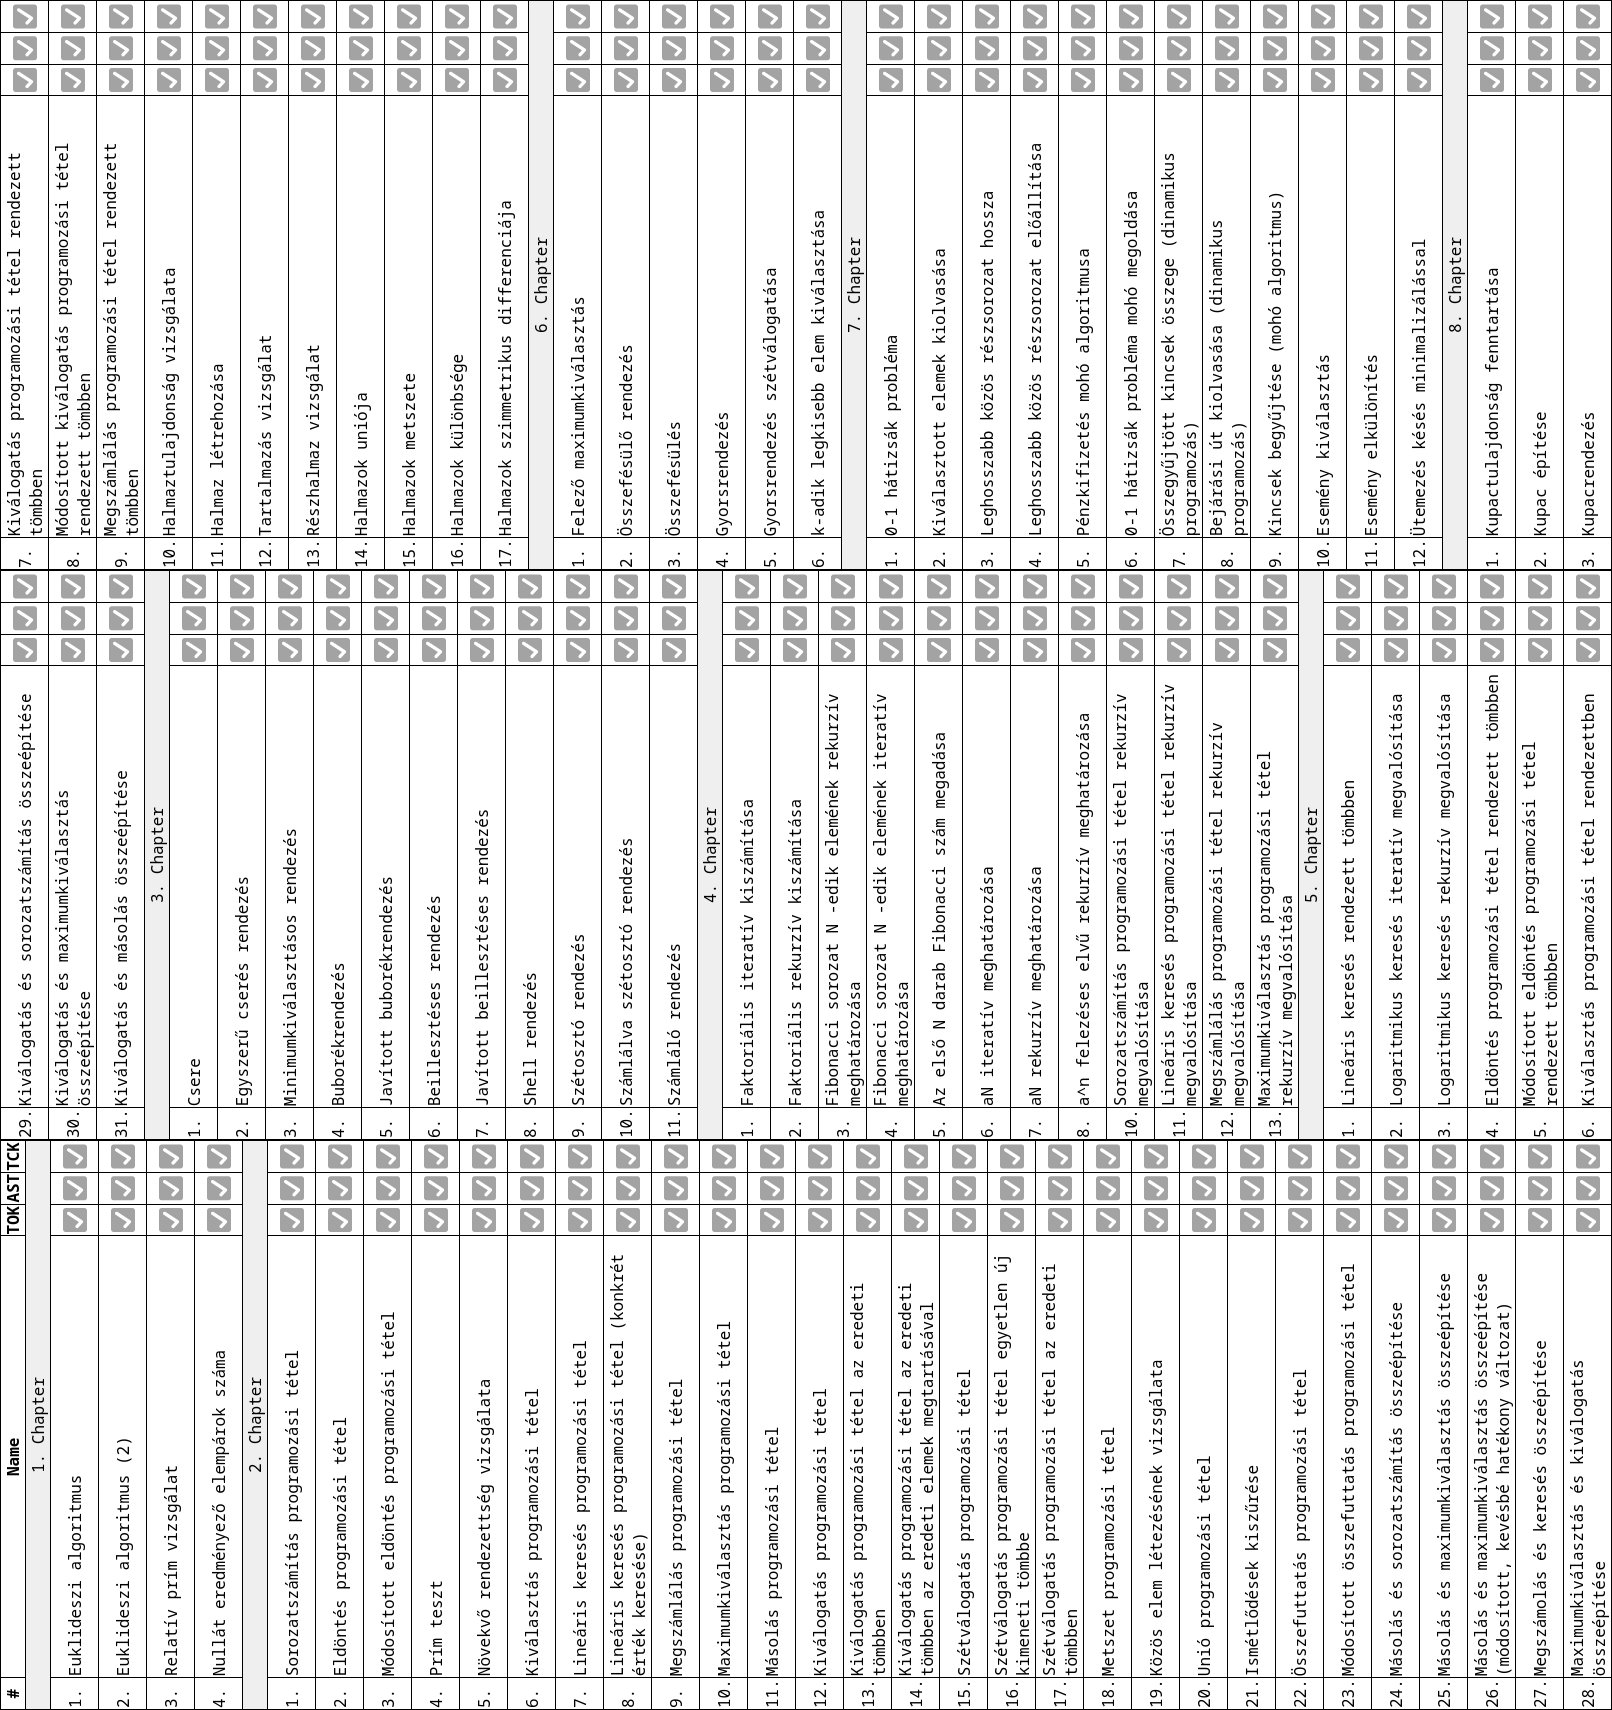
\includepdf[scale=0.9, offset=0.8cm -0.75cm, pagecommand=\section{MELLÉKLETEK}\subsection{Tesztelt algoritmusok listája}\label{algs}]{img/testing3.png}

\end{document}
